% Figure 10: Security Game Diagram
\documentclass[tikz,border=5pt]{standalone}
\usepackage{tikz}
\usetikzlibrary{arrows.meta,positioning,calc}

\begin{document}
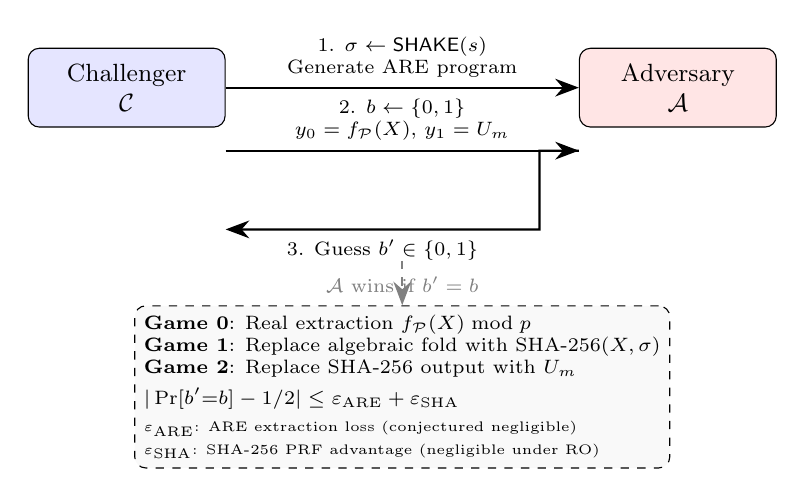
\begin{tikzpicture}[
  entity/.style={draw, rounded corners, minimum width=2.5cm, minimum height=1cm, align=center, font=\small},
  arr/.style={-{Stealth[length=3mm]}, thick},
  lbl/.style={font=\scriptsize, align=center},
]

% Challenger and Adversary
\node[entity, fill=blue!10] (C) at (0, 0) {Challenger\\$\mathcal{C}$};
\node[entity, fill=red!10] (A) at (7, 0) {Adversary\\$\mathcal{A}$};

% Game steps
\draw[arr] (C.east) -- node[above, lbl] {1. $\sigma \gets \mathsf{SHAKE}(s)$\\Generate ARE program} (A.west);

\draw[arr] ([yshift=-0.8cm]C.east) -- node[above, lbl] {2. $b \gets \{0,1\}$\\$y_0 = f_\mathcal{P}(X)$, $y_1 = U_m$} ([yshift=-0.8cm]A.west);

\draw[arr] ([yshift=-0.8cm]A.west) -- +(-0.5,0) -- +(-0.5,-1) -- node[below, lbl] {3. Guess $b' \in \{0,1\}$} ($(C.east) + (0,-1.8)$);

% Game hops
\node[draw, dashed, fill=gray!5, rounded corners, minimum width=5.5cm, align=left, font=\scriptsize] (hops) at (3.5, -3.8) {
  \textbf{Game 0}: Real extraction $f_\mathcal{P}(X) \bmod p$\\
  \textbf{Game 1}: Replace algebraic fold with SHA-256$(X, \sigma)$\\
  \textbf{Game 2}: Replace SHA-256 output with $U_m$\\[3pt]
  $|\Pr[b'{=}b] - 1/2| \leq \varepsilon_{\mathrm{ARE}} + \varepsilon_{\mathrm{SHA}}$\\[2pt]
  {\tiny $\varepsilon_{\mathrm{ARE}}$: ARE extraction loss (conjectured negligible)}\\
  {\tiny $\varepsilon_{\mathrm{SHA}}$: SHA-256 PRF advantage (negligible under RO)}
};

% Arrow to game hops
\draw[arr, dashed, gray] (3.5, -2.2) -- (hops.north);

% Outcome
\node[font=\scriptsize, text=gray] at (3.5, -2.5) {$\mathcal{A}$ wins if $b' = b$};

\end{tikzpicture}
\end{document}
